%% fig_efourthree.tex   (generated by make_round43.py; do not edit by hand)
%% Three consecutive shifts on E_0^8: blocks, targets, budget and spectrum (thm:efourthreelevels).
\documentclass[tikz,border=8pt]{standalone}
\usepackage{amsmath,amssymb}
\usetikzlibrary{arrows.meta,calc,decorations.pathreplacing}
%% palette.tex -- shared colour definitions for the figures
\definecolor{PInk}{RGB}{26,32,44}
\definecolor{PBlue}{RGB}{37,82,139}
\definecolor{PTeal}{RGB}{23,127,125}
\definecolor{POchre}{RGB}{193,138,44}
\definecolor{PClay}{RGB}{178,74,58}
\definecolor{PSlate}{RGB}{108,122,137}
\definecolor{PViolet}{RGB}{110,86,150}
\definecolor{WBlue}{RGB}{223,234,246}
\definecolor{WTeal}{RGB}{220,238,236}
\definecolor{WOchre}{RGB}{250,240,218}
\definecolor{WClay}{RGB}{247,229,224}
\definecolor{WSlate}{RGB}{238,241,244}
\definecolor{PMag}{RGB}{158,58,110}
\definecolor{PGrass}{RGB}{62,124,66}
\definecolor{PAmber}{RGB}{214,112,38}
\definecolor{PIndigo}{RGB}{58,64,140}
\definecolor{PRule}{RGB}{176,186,197}

%% shared macros so the standalone figures match the paper
\providecommand{\QQ}{\mathbb{Q}}
\providecommand{\ZZ}{\mathbb{Z}}
\providecommand{\RR}{\mathbb{R}}
\providecommand{\CC}{\mathbb{C}}
\providecommand{\PP}{\mathbb{P}}
\providecommand{\Kx}{K^{\times}}
\providecommand{\HW}{W}
\providecommand{\Nm}{\mathrm{N}}
\providecommand{\Hdg}{\mathrm{Hdg}}
\providecommand{\NS}{\mathrm{NS}}
\providecommand{\cA}{\mathcal{A}}
\providecommand{\cD}{\mathcal{D}}
\providecommand{\cF}{\mathcal{F}}
\providecommand{\cP}{\mathcal{P}}
\providecommand{\cO}{\mathcal{O}}
\providecommand{\cQ}{\mathcal{Q}}
\providecommand{\bbar}[1]{\overline{#1}}
\providecommand{\ch}{\operatorname{ch}}
\providecommand{\End}{\mathrm{End}}
\providecommand{\Ext}{\operatorname{Ext}}
\providecommand{\Supp}{\operatorname{Supp}}

\begin{document}
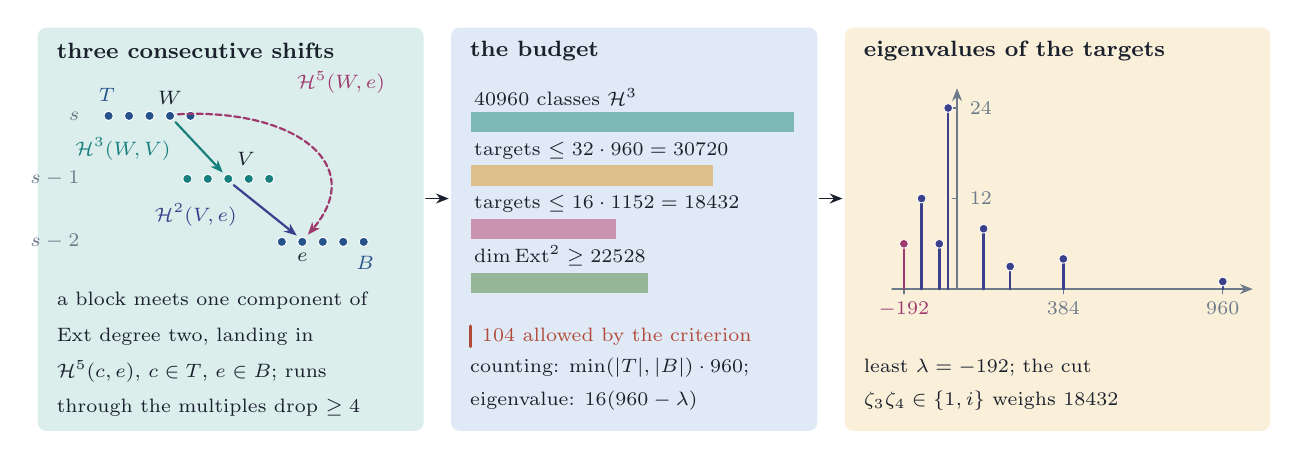
\begin{tikzpicture}[x=1cm,y=1cm,line join=round,line cap=round,
  font=\small,text=PInk,lbl/.style={inner sep=1pt}]
  \path[fill=WTeal,draw=none,rounded corners=3.0pt] (0.0500,-0.5000) rectangle (4.9500,4.6200);
  \path[fill=WBlue,draw=none,rounded corners=3.0pt] (5.3000,-0.5000) rectangle (9.9500,4.6200);
  \path[fill=PTeal!55!white,draw=none] (5.5500,3.2900) rectangle (9.6500,3.5500);
  \path[fill=POchre!55!white,draw=none] (5.5500,2.6100) rectangle (8.6250,2.8700);
  \path[fill=PMag!55!white,draw=none] (5.5500,1.9300) rectangle (7.3950,2.1900);
  \path[fill=PGrass!55!white,draw=none] (5.5500,1.2500) rectangle (7.8050,1.5100);
  \path[fill=WOchre,draw=none,rounded corners=3.0pt] (10.3000,-0.5000) rectangle (15.7000,4.6200);
  \path[fill=PBlue,draw=white,line width=0.35pt] (0.9500,3.5000) circle (1.70pt);
  \path[fill=PBlue,draw=white,line width=0.35pt] (1.2100,3.5000) circle (1.70pt);
  \path[fill=PBlue,draw=white,line width=0.35pt] (1.4700,3.5000) circle (1.70pt);
  \path[fill=PBlue,draw=white,line width=0.35pt] (1.7300,3.5000) circle (1.70pt);
  \path[fill=PBlue,draw=white,line width=0.35pt] (1.9900,3.5000) circle (1.70pt);
  \path[fill=PTeal,draw=white,line width=0.35pt] (1.9500,2.7000) circle (1.70pt);
  \path[fill=PTeal,draw=white,line width=0.35pt] (2.2100,2.7000) circle (1.70pt);
  \path[fill=PTeal,draw=white,line width=0.35pt] (2.4700,2.7000) circle (1.70pt);
  \path[fill=PTeal,draw=white,line width=0.35pt] (2.7300,2.7000) circle (1.70pt);
  \path[fill=PTeal,draw=white,line width=0.35pt] (2.9900,2.7000) circle (1.70pt);
  \path[fill=PBlue,draw=white,line width=0.35pt] (3.1500,1.9000) circle (1.70pt);
  \path[fill=PBlue,draw=white,line width=0.35pt] (3.4100,1.9000) circle (1.70pt);
  \path[fill=PBlue,draw=white,line width=0.35pt] (3.6700,1.9000) circle (1.70pt);
  \path[fill=PBlue,draw=white,line width=0.35pt] (3.9300,1.9000) circle (1.70pt);
  \path[fill=PBlue,draw=white,line width=0.35pt] (4.1900,1.9000) circle (1.70pt);
  \draw[PTeal,line width=0.8pt,-{Stealth[length=4.6pt,width=3.6pt]}] (1.8000,3.4200) -- (2.4000,2.7800);
  \draw[PIndigo,line width=0.8pt,-{Stealth[length=4.6pt,width=3.6pt]}] (2.5400,2.6200) -- (3.3400,1.9800);
  \draw[PMag,line width=0.8pt,dash pattern=on 2.2pt off 1.2pt,-{Stealth[length=4.6pt,width=3.6pt]}] (1.8300,3.5200) .. controls (3.2800,3.6000) and (4.2600,2.9000) .. (3.4800,1.9900);
  \draw[PClay,line width=1.2pt] (5.5500,0.5700) -- (5.5500,0.8300);
  \draw[PSlate,line width=0.5pt,-{Stealth[length=4.6pt,width=3.6pt]}] (10.9000,1.3000) -- (15.4800,1.3000);
  \draw[PSlate,line width=0.5pt,-{Stealth[length=4.6pt,width=3.6pt]}] (11.7250,1.3000) -- (11.7250,3.8500);
  \draw[PSlate,line width=0.5pt] (11.0500,1.3000) -- (11.0500,1.2400);
  \draw[PSlate,line width=0.5pt] (13.0750,1.3000) -- (13.0750,1.2400);
  \draw[PSlate,line width=0.5pt] (15.1000,1.3000) -- (15.1000,1.2400);
  \draw[PSlate,line width=0.5pt] (11.6650,2.4500) -- (11.7250,2.4500);
  \draw[PSlate,line width=0.5pt] (11.6650,3.6000) -- (11.7250,3.6000);
  \draw[PMag,line width=0.9pt] (11.0500,1.3000) -- (11.0500,1.8750);
  \path[fill=PMag,draw=white,line width=0.30pt] (11.0500,1.8750) circle (1.60pt);
  \draw[PIndigo,line width=0.9pt] (11.2750,1.3000) -- (11.2750,2.4500);
  \path[fill=PIndigo,draw=white,line width=0.30pt] (11.2750,2.4500) circle (1.60pt);
  \draw[PIndigo,line width=0.9pt] (11.5000,1.3000) -- (11.5000,1.8750);
  \path[fill=PIndigo,draw=white,line width=0.30pt] (11.5000,1.8750) circle (1.60pt);
  \draw[PIndigo,line width=0.9pt] (11.6125,1.3000) -- (11.6125,3.6000);
  \path[fill=PIndigo,draw=white,line width=0.30pt] (11.6125,3.6000) circle (1.60pt);
  \draw[PIndigo,line width=0.9pt] (12.0625,1.3000) -- (12.0625,2.0667);
  \path[fill=PIndigo,draw=white,line width=0.30pt] (12.0625,2.0667) circle (1.60pt);
  \draw[PIndigo,line width=0.9pt] (12.4000,1.3000) -- (12.4000,1.5875);
  \path[fill=PIndigo,draw=white,line width=0.30pt] (12.4000,1.5875) circle (1.60pt);
  \draw[PIndigo,line width=0.9pt] (13.0750,1.3000) -- (13.0750,1.6833);
  \path[fill=PIndigo,draw=white,line width=0.30pt] (13.0750,1.6833) circle (1.60pt);
  \draw[PIndigo,line width=0.9pt] (15.1000,1.3000) -- (15.1000,1.3958);
  \path[fill=PIndigo,draw=white,line width=0.30pt] (15.1000,1.3958) circle (1.60pt);
  \draw[PInk,line width=0.6pt,-{Stealth[length=4.6pt,width=3.6pt]}] (4.9800,2.4500) -- (5.2700,2.4500);
  \draw[PInk,line width=0.6pt,-{Stealth[length=4.6pt,width=3.6pt]}] (9.9800,2.4500) -- (10.2700,2.4500);
  \node[lbl,anchor=west,text=PInk,font=\footnotesize] at (0.2500,4.3200) {\textbf{three consecutive shifts}};
  \node[lbl,anchor=east,text=PSlate,font=\scriptsize] at (0.6200,3.5000) {$s$};
  \node[lbl,anchor=east,text=PSlate,font=\scriptsize] at (0.6200,2.7000) {$s-1$};
  \node[lbl,anchor=east,text=PSlate,font=\scriptsize] at (0.6200,1.9000) {$s-2$};
  \node[lbl,anchor=south,text=PBlue,font=\scriptsize] at (0.9300,3.6400) {$T$};
  \node[lbl,anchor=north,text=PBlue,font=\scriptsize] at (4.2100,1.7600) {$B$};
  \node[lbl,anchor=east,text=PTeal,font=\scriptsize] at (1.7800,3.0800) {$\mathcal{H}^{3}(W,V)$};
  \node[lbl,anchor=east,text=PIndigo,font=\scriptsize] at (2.6200,2.2400) {$\mathcal{H}^{2}(V,e)$};
  \node[lbl,anchor=west,text=PMag,font=\scriptsize] at (3.3000,3.9226) {$\mathcal{H}^{5}(W,e)$};
  \node[lbl,anchor=south,text=PInk,font=\scriptsize] at (1.7300,3.6000) {$W$};
  \node[lbl,anchor=west,text=PInk,font=\scriptsize] at (2.5400,2.9562) {$V$};
  \node[lbl,anchor=north,text=PInk,font=\scriptsize] at (3.4100,1.8000) {$e$};
  \node[lbl,anchor=west,text=PInk,font=\scriptsize] at (0.2500,1.1500) {a block meets one component of};
  \node[lbl,anchor=west,text=PInk,font=\scriptsize] at (0.2500,0.7000) {$\Ext$ degree two, landing in};
  \node[lbl,anchor=west,text=PInk,font=\scriptsize] at (0.2500,0.2500) {$\mathcal{H}^{5}(c,e)$, $c\in T$, $e\in B$; runs};
  \node[lbl,anchor=west,text=PInk,font=\scriptsize] at (0.2500,-0.2000) {through the multiples drop $\ge4$};
  \node[lbl,anchor=west,text=PInk,font=\footnotesize] at (5.5000,4.3200) {\textbf{the budget}};
  \node[lbl,anchor=west,text=PInk,font=\scriptsize] at (5.5500,3.7418) {$40960$ classes $\mathcal{H}^{3}$};
  \node[lbl,anchor=west,text=PInk,font=\scriptsize] at (5.5500,3.0604) {targets $\le32\cdot960=30720$};
  \node[lbl,anchor=west,text=PInk,font=\scriptsize] at (5.5500,2.3804) {targets $\le16\cdot1152=18432$};
  \node[lbl,anchor=west,text=PInk,font=\scriptsize] at (5.5500,1.7246) {$\dim\Ext^{2}\ge22528$};
  \node[lbl,anchor=west,text=PClay,font=\scriptsize] at (5.6500,0.7000) {$104$ allowed by the criterion};
  \node[lbl,anchor=west,text=PInk,font=\scriptsize] at (5.5000,0.3000) {counting: $\min(|T|,|B|)\cdot960$;};
  \node[lbl,anchor=west,text=PInk,font=\scriptsize] at (5.5000,-0.1200) {eigenvalue: $16(960-\lambda)$};
  \node[lbl,anchor=west,text=PInk,font=\footnotesize] at (10.5000,4.3200) {\textbf{eigenvalues of the targets}};
  \node[lbl,anchor=north,text=PMag,font=\scriptsize] at (11.0500,1.1800) {$-192$};
  \node[lbl,anchor=north,text=PSlate,font=\scriptsize] at (13.0750,1.1800) {$384$};
  \node[lbl,anchor=north,text=PSlate,font=\scriptsize] at (15.1000,1.1800) {$960$};
  \node[lbl,anchor=west,text=PSlate,font=\scriptsize] at (11.8450,2.4500) {$12$};
  \node[lbl,anchor=west,text=PSlate,font=\scriptsize] at (11.8450,3.6000) {$24$};
  \node[lbl,anchor=west,text=PInk,font=\scriptsize] at (10.5000,0.3000) {least $\lambda=-192$; the cut};
  \node[lbl,anchor=west,text=PInk,font=\scriptsize] at (10.5000,-0.1200) {$\zeta_{3}\zeta_{4}\in\{1,i\}$ weighs $18432$};
\end{tikzpicture}
\end{document}
